
\chapter{Avoiding Unprofitable Merge Operations with Deep Learning} \label{chp:deeplearning}

Chapter~\ref{chp:cgo19} describes our strategy for ranking the function candidates that are more likely to be profitably merged.
However, most of the merged functions are actually unprofitable candidates, since many functions are unique enough to have no profitable paring.
Even if we consider only the top candidate functions, only about 13\% result in a profitable merge operation.

Since the function merging operation is computationally expensive, ideally we need to focus our effort only to those are most likely to be profitable and avoid wastefully merging unprofitable pairs of functions.
In this chapter, we describe our heuristic model based on deep-learning to predict whether a pair of functions can be
profitably merged or not.
This allows us to avoid merging pairs of functions that are unlikely to result in a profitable merge operation.

\section{Motivation} \label{sec:deeplearning:motivation}

In this section, we discuss two weaknesses in our current function merging optimization.
First, we show that there is a significant opportunity in reduction that can be gained by having a better profitability analysis.
%Second, we show that we can save compilation time by bailing out early from unprofitable merge operations, avoiding wasteful merges.
Second, we show that most function merging attempts are thrown away as they cause code bloat, according to the profitability analysis.

\subsection{Inaccuracies in the Profitability Analysis}

Although the proposed technique is able to merge any two functions, it is not always profitable to do so.
A pair of functions can be profitably merged when replacing them by the merged function results in an overall smaller code.
As it is only profitable to merge functions that are sufficiently similar, for most pairs of functions, merging them increases code size.
Since the profitability analysis is critical for the optimisation strategy, we must be able to effectively decide which pair of functions can be profitably merged.

In order to estimate the code-size benefit, we first estimate the size of all three functions, i.e., the two input functions and the merged one.
The size of each function is estimated by summing up the estimated binary size of all instruction in the function, in its IR form.
The binary size of each IR instruction is estimated by querying the compiler's built-in target-specific cost model.
These cost models provide target-dependent cost estimations approximating the code-size cost of an IR instruction when lowered to machine instructions.

As pointed out by many prior work~\cite{porpodas18,rocha19,rocha20}, even though cost models offer a good trade-off between compilation time and accuracy, they are expected to contain inaccuracies.
Because we are trying to estimate the binary size of the final object code, inaccuracies arise from the fact that we are operating on the IR level and one IR instruction does not necessarily translate to one machine instruction.
Because we are operating on the IR level, We cannot know exactly how each IR instruction will be lowered without actually running the compiler's backend.
Moreover, several number of optimisations and code transformations will still run prior to machine code generation.
%The same IR instruction can be lowered to different machine instructions, depending on its surrounding context, the instruction selection algorithm, and many other factors.
%Therefore, there is also an inherent limitation of estimating the cost of each instruction separately of its context.

Figure~\ref{fig:oracle-reduction} presents the code size reduction that can be achieved with an oracle.
This oracle measures code size by compiling the whole program down to its final object file, which provides perfect information for the cost model.
It shows the potential for improvement there exists from having a better profitability analysis, almost doubling the reduction.
By compiling the whole program down to its binary form, we are able to precisely capture the impact on other optimizations and machine code generation, as well as the overheads that result from replacing the callsites to the merged function or keeping a \textit{thunk}.

\begin{figure}[h]
  \centering
  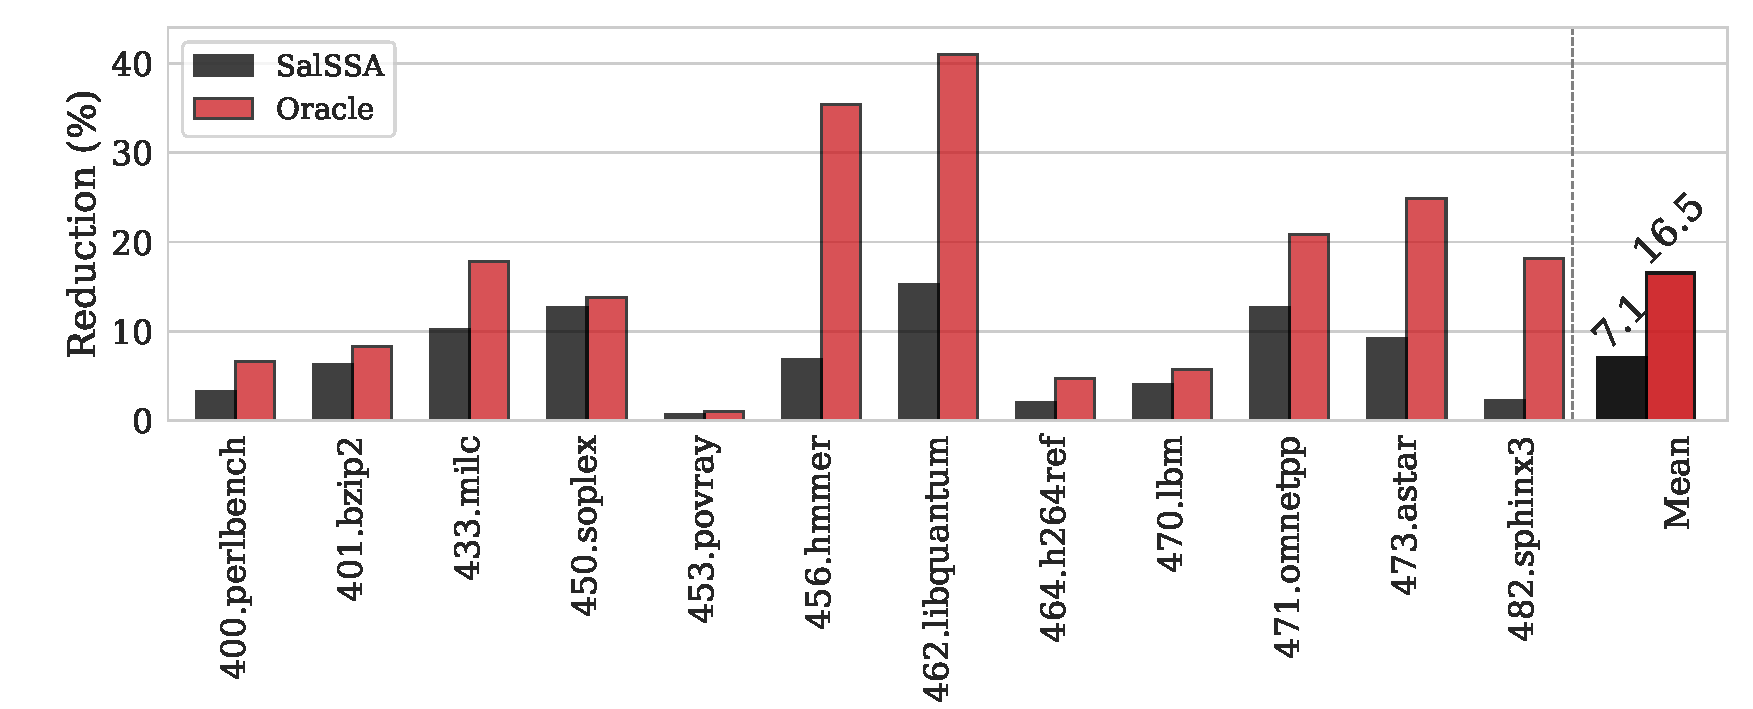
\includegraphics[width=0.8\textwidth]{src/deeplearning/figs/motivation-oracle-reduction.pdf}
  \caption{.}
  \label{fig:oracle-reduction}
\end{figure}

However, the cost of compiling the whole program for every merging attempt is prohibitive.
The re-compilation overhead can be severely aggravated for larger programs with multiple functions, where not only each compilation takes longer but the whole program is also re-compiled many times.

\subsection{Wasteful Merge Operations}

The fingerprint-based ranking strategy helps the function merging optimization to pair functions that are more similar.
However, the current strategy is unable to decide which one of those pairs are actually worth merging.
Figure~\ref{fig:unprofitable-attempts} shows that about 82\% of the top ranked candidate functions are actually unprofitably merged.
As a result, a considerable amount of compilation time is wasted producing merged functions that will be thrown away, keeping the original pair of functions.

\begin{figure}[h]
  \centering
  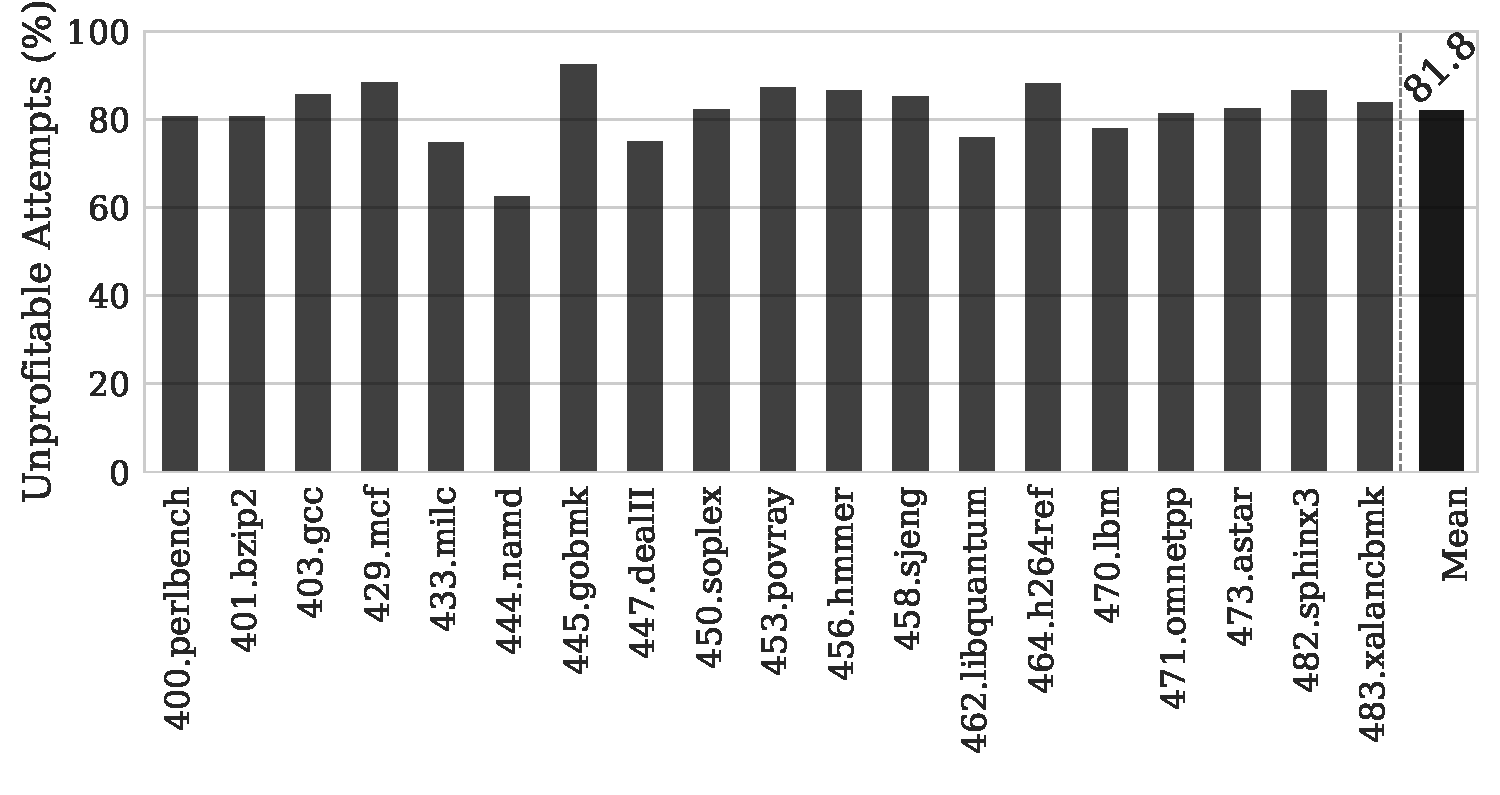
\includegraphics[width=0.8\textwidth]{src/deeplearning/figs/unprofitable-attempts.pdf}
  \caption{An average of about 82\% of merging attempts are unprofitable.}
  \label{fig:unprofitable-attempts}
\end{figure}

%Figure~\ref{fig:compilation-breakdown} shows a breakdown of the time spent in different steps of the function merging optimization.
%As expected, this breakdown confirms that most of the compilation-time is spent merging functions, which includes both the sequence alignment and code generation.
%This also includes the time wasted producing unprofitable merged functions.
%Therefore, it is important to avoid merging unprofitable functions.

%Figure~\ref{fig:unprofitable-compile-time-percentage} shows the time spent producing unprofitable merged functions relative to the total compilation time of the function merging optimization.
Since most of the merged functions are thrown away for being unprofitable, it is expected that most of the compilation time is also spent producing those merged functions.
This impact is also aggravated when several of the unprofitable merged functions are much larger than the profitable ones.
Therefore, it is of utmost importance that we avoid merging unprofitable functions.
If we could eliminate all the time wasted on unprofitable merge operations, we would free compilation time for more useful computation.

%\begin{figure}[h]
%  \centering
%  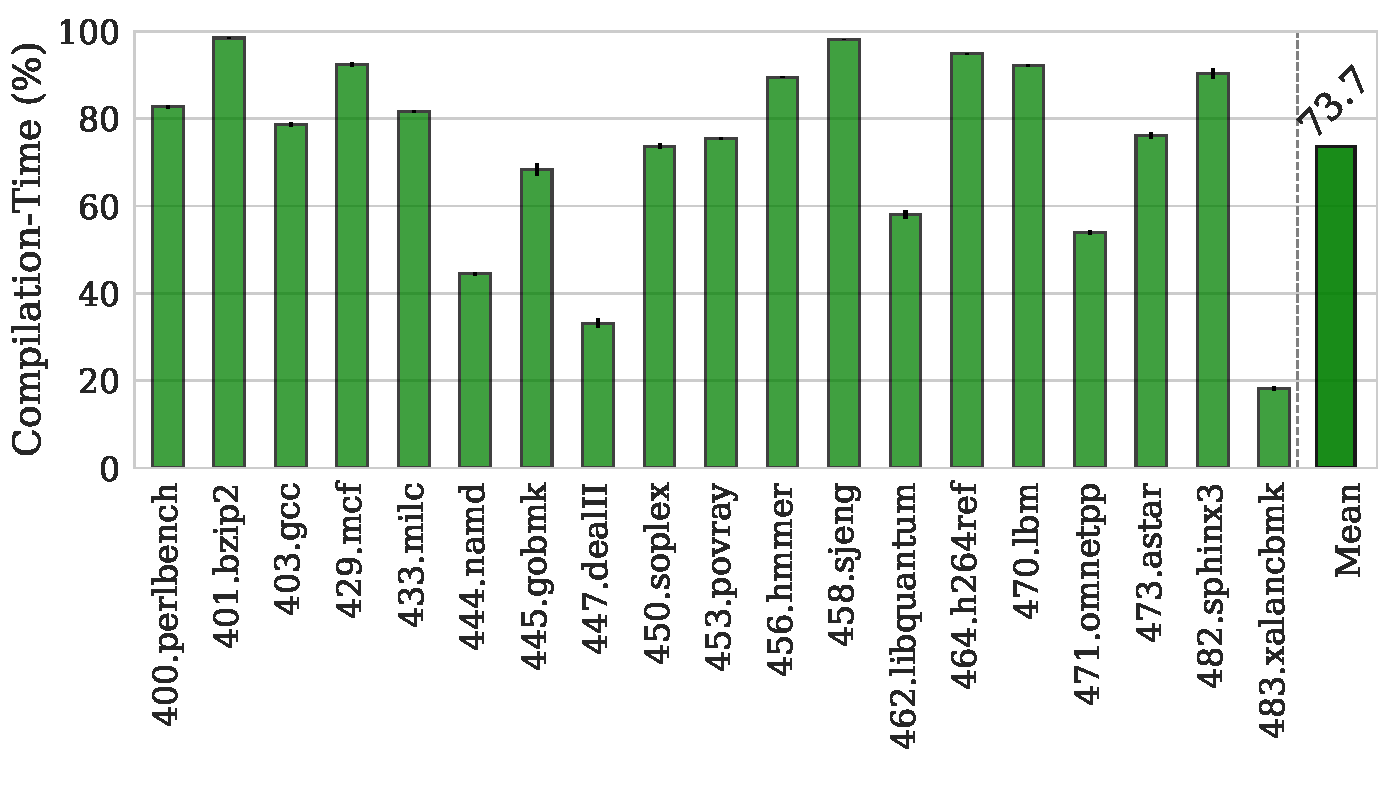
\includegraphics[width=0.8\textwidth]{src/deeplearning/figs/unprofitable-compile-time-percentage.pdf}
%  \caption{The percentage of compilation-time spent on unprofitable merge operations.}
%  \label{fig:unprofitable-compile-time-percentage}
%\end{figure}


\subsection{Summary}

In this paper, our goal is to develop a solution capable of identifying whether or not a given pair of functions can be profitably merged, allowing us to use a more expensive profitability analysis based on partial re-compilation.
If we could predict which pairs of function are more likely to cause code bloat, we could avoid wasting time merging them in the first place and having to estimate their binary sizes.
Bailing out early frees time to be spent on more profitable merge operations.





\section{Our Novel Profitability Analysis}

\subsection{Realistic Code-Size Cost} \label{sec:recompilation-mechanism}

In Section~\ref{sec:deeplearning:motivation}, we describe the limitations of code size estimation using existing compiler's cost models.
In our motivation, we use an oracle cost model, with perfect information, that can be obtained by recompiling the whole program in order to decide which version produces a smaller binary.
However, this solution is infeasible due to compilation time overheads.
Large programs with thousands of functions can take days to optimise due to the excessive number of long recompilations, sometimes taking up to a couple days.

In this section, we propose a novel approach based on partial recompilation.
This approach is capable of significantly reducing the compilation time required by the oracle cost model, while still providing equivalent benefits.

%Our goal is to be able to capture the changes in the code that result from merging a pair of functions.
Our goal is to extract to a separate module only the code that can be potentially affected by merging a given pair of functions.
Beyond the difference in size of the merged function itself, code size can also be affected by the need for a thunk that calls the merged function while preserving the original interface.
Call-sites updated to call the merged function require extra arguments which might affect code-size directly or indirectly. %%i.e., higher register pressure
Finally, inter-procedural analyses and optimisations can have their decision making altered by the merged function.

In order to capture all the possible ways that function merging can influence code size, we extract to a different module the functions being merged as well as their user functions, such as callers or functions that take their address.
We also need to extract all global definitions and variables referenced by any of these functions, which include the declaration or signature of functions called by any of them.
Figure~\ref{fig:our-cost-model-callgraph-1} illustrates an example of code extracted by our partial recompilation approach.

\begin{figure}[h]
\centering
\begin{subfigure}{\textwidth}
  \centering
  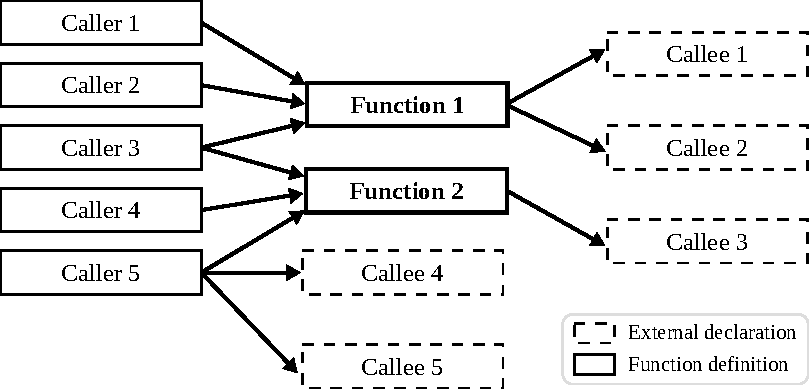
\includegraphics[scale=0.8]{src/deeplearning/figs/our-cost-model-callgraph-1.pdf}
  \caption{Extracted code without function merging.}
  \label{fig:our-cost-model-callgraph-1}
\end{subfigure}
\\
\begin{subfigure}{\textwidth}
\centering
  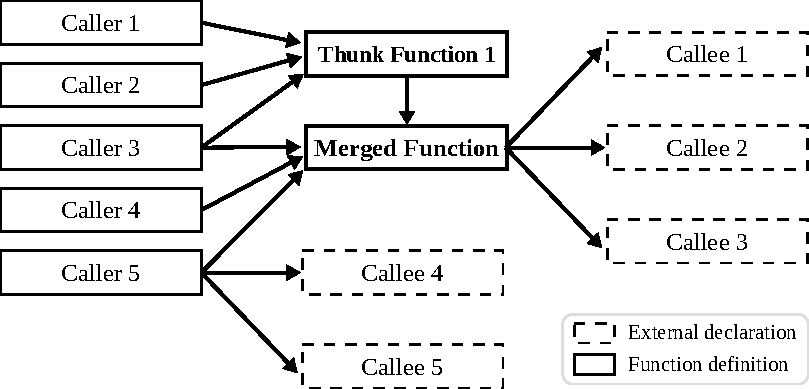
\includegraphics[scale=0.8]{src/deeplearning/figs/our-cost-model-callgraph-2.pdf}
  \caption{Extracted code with function merging.}
  \label{fig:our-cost-model-callgraph-2}
\end{subfigure}
\caption{Example of the code extracted to compare the binary size before and after function merging, in order to decide whether or not it is profitable to merge a given pair of functions.}
\label{fig:our-cost-model-callgraphs}
\end{figure}

After compiling and measuring the size of the extracted code, we then apply the changes caused by merging the given pair of functions, as illustrated in Figure~\ref{fig:our-cost-model-callgraph-2}.
These changes represent the real impact function merging would cause in the real program.
Once the function merging has been applied, the code is recompiled.
If function merging produces a smaller binary, then these changes are also applied to the real program.
%As shown in Figure~\ref{fig:our-cost-model-callgraph-2}, when applying function merging to the extracted code, it is able to 

\subsection{Learning a Profitability Model} \label{sec:deepprofit-model}

\begin{figure}[h]
  \centering
  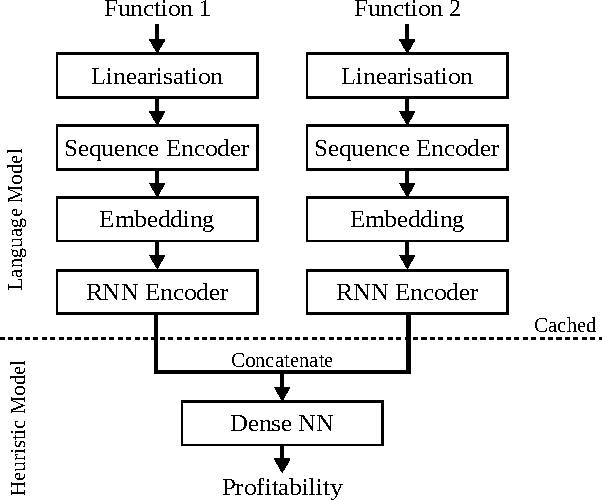
\includegraphics[width=0.65\textwidth]{src/deeplearning/figs/deeplearning-architecture.pdf}
  \caption{
      The proposed deep-learning model architecture that predicts which pairs of functions will be profitably merged. Code properties are extracted from each function into \textit{context vectors} by the language model.
      These context vectors are cached to be later fed to the heuristic model to produce the final profitability prediction.}
  \label{fig:heuristic-model-architecture}
\end{figure}

Figure~\ref{fig:heuristic-model-architecture} provides an overview of the prediction mechanism.
Our mechanism follows a similar approach to previous deep-learning techniques for tuning compilers~\cite{cummins17, mendis19}.

The same linearised functions used for the merge operations, as described in Chapter~\ref{chp:fm-operation}, are used as input to the prediction model.
First, we use a language model based on recurrent neural networks to encode the input functions into context vectors of fixed size.
These vector encodings can be computed only once per function an cached.
Finally, the context vectors of two input functions are concatenated and fed to a feed-forward neural network that classifies whether or not those functions are profitably merged.

\subsection{Search Strategy}

\begin{figure}[h]
  \centering
  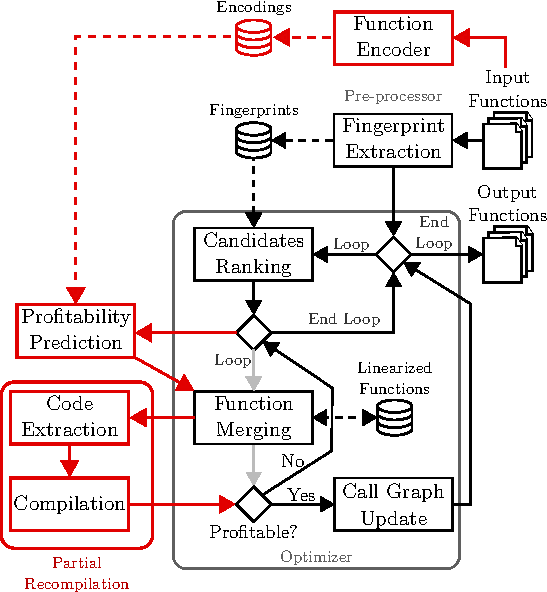
\includegraphics[width=0.65\textwidth]{src/deeplearning/figs/func-merge-opt-new-arch.pdf}
  \caption{Overview of our extended exploration framework.}
  \label{fig:func-merge-opt-new-arch}
\end{figure}

Figure~\ref{fig:func-merge-opt-new-arch} shows how we extend the search strategy described in Section~\ref{sec:framework}.
We keep the fingerprint-based ranking mechanism, from the original strategy, that avoids a prohibitive quadratic exploration over all pairs of functions.
For each function, a priority queue is used to rank the topmost similar candidates on a fingerprint-based distance metric.
A greedy exploration is performed on the topmost similar candidates up to a threshold limit, terminating after finding the first candidate that results in a profitable merge and committing that merge operation.
Unlike the prior profitability analysis that simply used the built-in compiler cost model, the new search strategy has a two-tier approach with increasing accuracy and computational cost.

The first-tier is the ML-based approach described in Section~\ref{sec:deepprofit-model}.
The main goal of the first-tier is to avoid going to the highly expensive second-tier for clearly unprofitable pairs of input functions. 
First, we pre-compute a fixed-length encoding for every function, using a recurrent neural network.
Similar to the fingerprints, these fixed-length encodings need only be computed once for each function.
During the actual search, the encodings of the input pair of functions are then fed into a binary-classifier that predicts the profitability of merging those functions.
Only the positive predictions move forward to the second-tier.

The second-tier is the partial recompilation mechanism described in Section~\ref{sec:recompilation-mechanism}.
This is an accurate but expensive profitability analysis.
It requires the compilation of the input functions as well as the merged function, in order to know their final binary size.
If the object file containing the merged function is smaller than the alternative, the merged function is committed, otherwise we rollback to the original version with both input functions.

\section{Evaluation}

%\begin{figure*}[h]
%  \centering
%  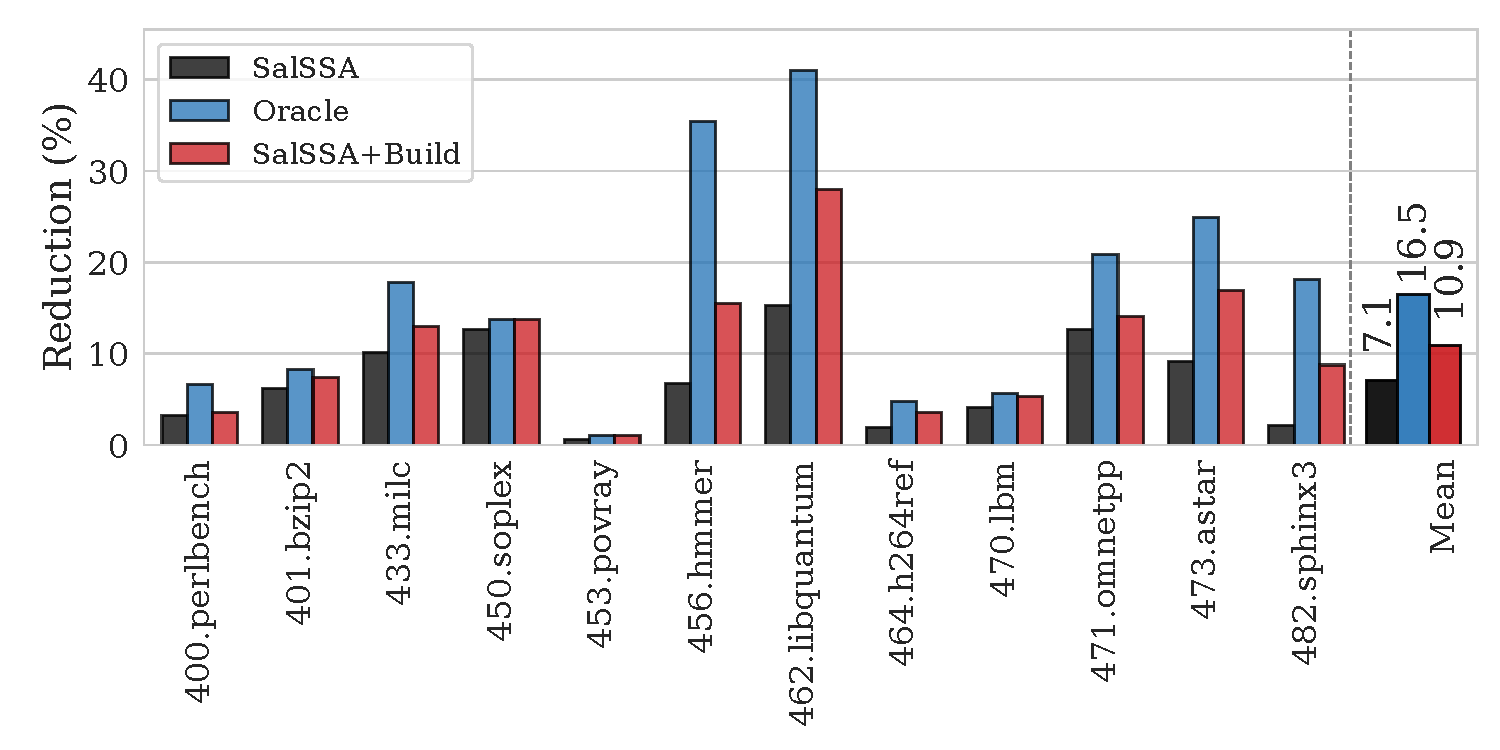
\includegraphics[width=\textwidth]{src/deeplearning/figs/code-size-oracle-vs-partial.pdf}
%  \vspace{-2.5em}
%  \caption{.}
%  \label{fig:code-size-oracle-vs-partial}
%\end{figure*}


%\begin{figure*}[h]
%  \centering
%  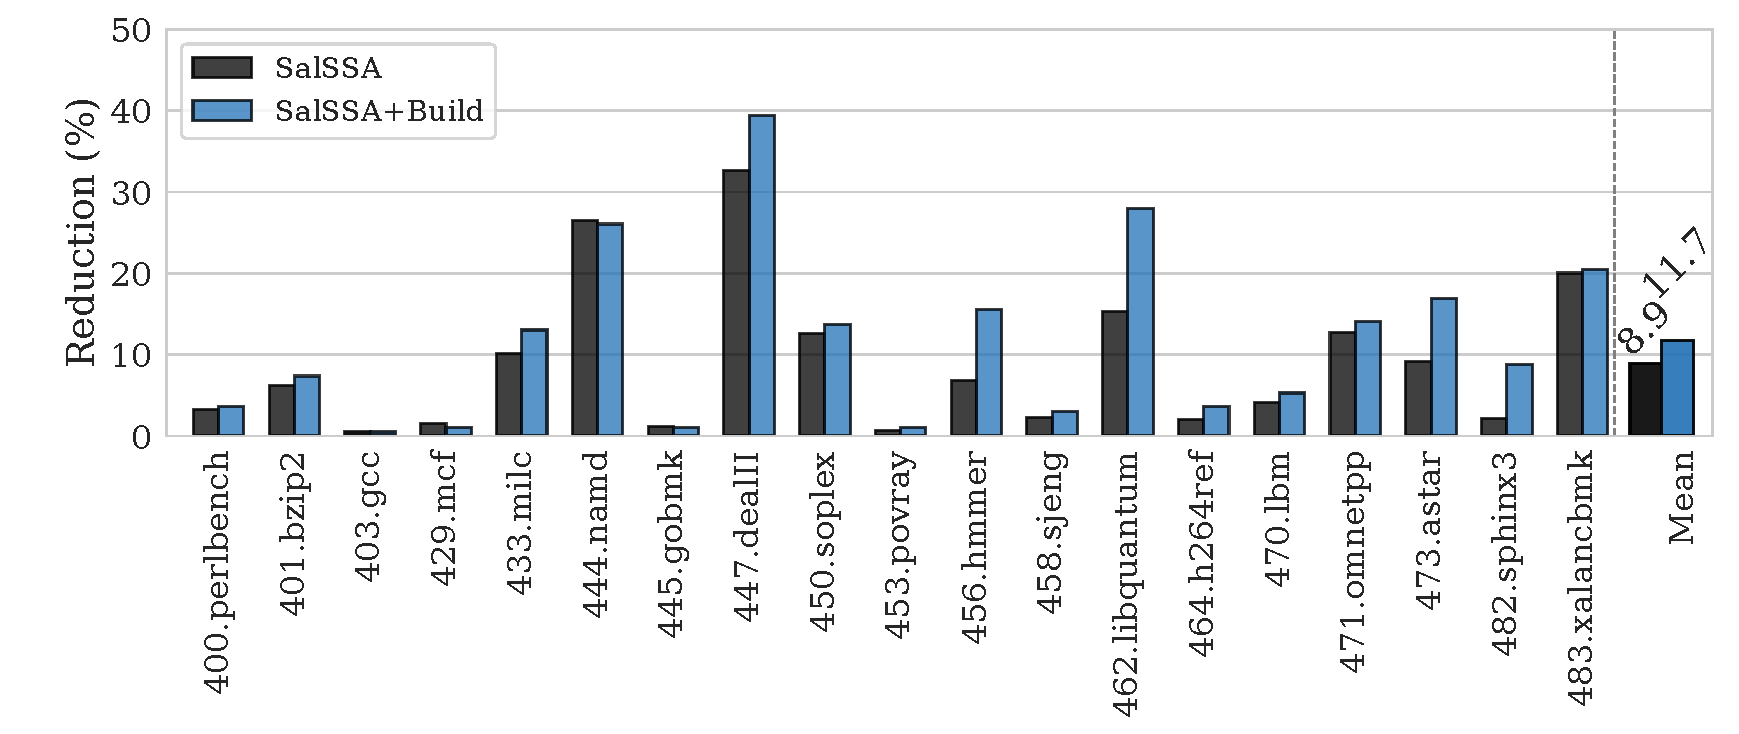
\includegraphics[width=\textwidth]{src/deeplearning/figs/code-size-partial.pdf}
%  \vspace{-2.5em}
%  \caption{.}
%  \label{fig:code-size-partial}
%\end{figure*}

Figure~\ref{fig:prediction-ss} shows the evaluation of both the \textit{sensitivity} and \textit{specificity} of our ML-based profitability classifier.
Essentially, the \textit{sensitivity} (true-positive rate) translates to code-size reduction as it represents the identification of actually profitable functions. 
\textit{Specificity} (true-negative rate) translates directly to fewer recompilations as it represents unprofitable functions being ignored.

\begin{figure*}[h]
  \centering
  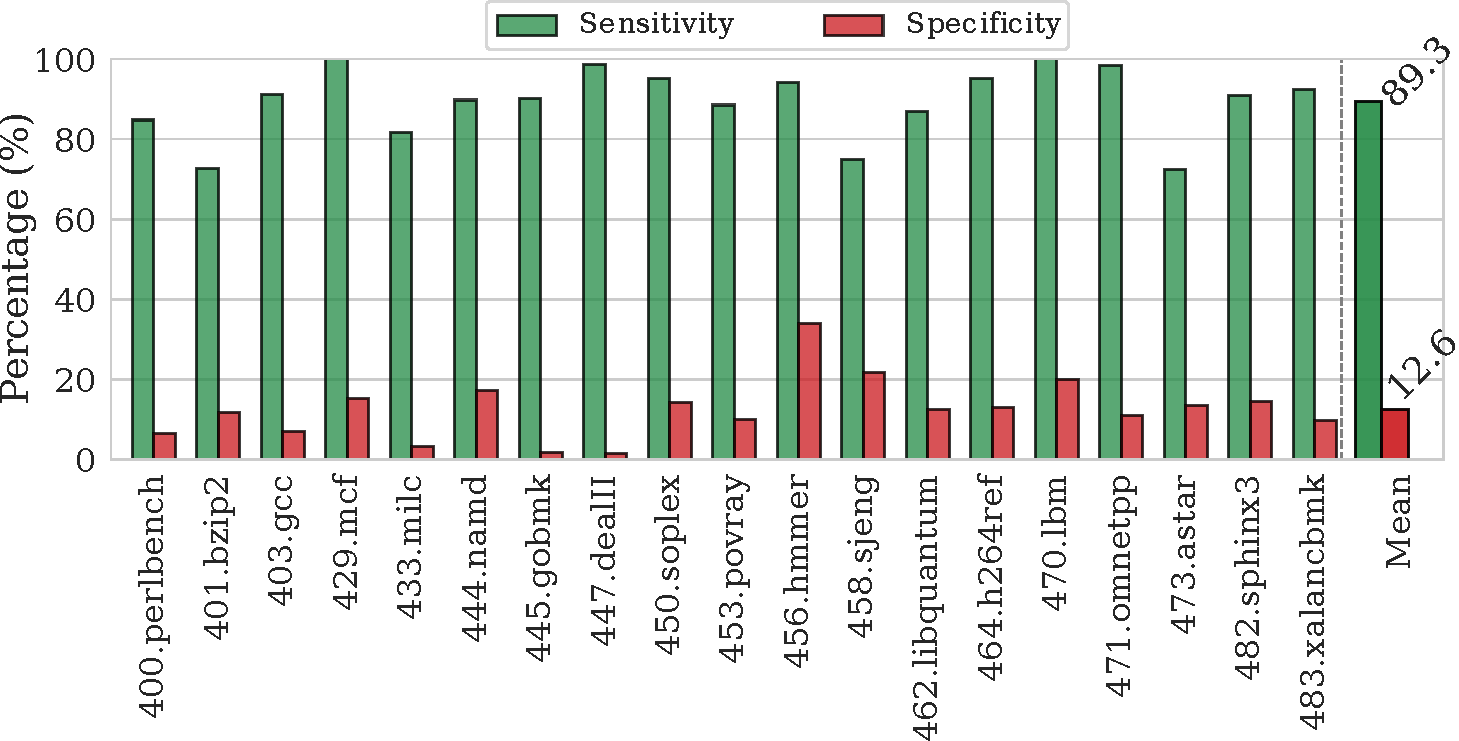
\includegraphics[width=0.85\textwidth]{src/deeplearning/figs/prediction-ss.pdf}
  \caption{Evaluation of the \textit{sensitivity} (true-positive rate) and \textit{specificity} (true-negative rate) of our profitability classifier.
  Sensitivity represents all profitable merging attempts that our model correctly identifies. 
  Specificity represents how many unprofitable merging attempts our predictive model is able to avoid.
  }
  \label{fig:prediction-ss}
\end{figure*}


\begin{figure*}[h]
  \centering
  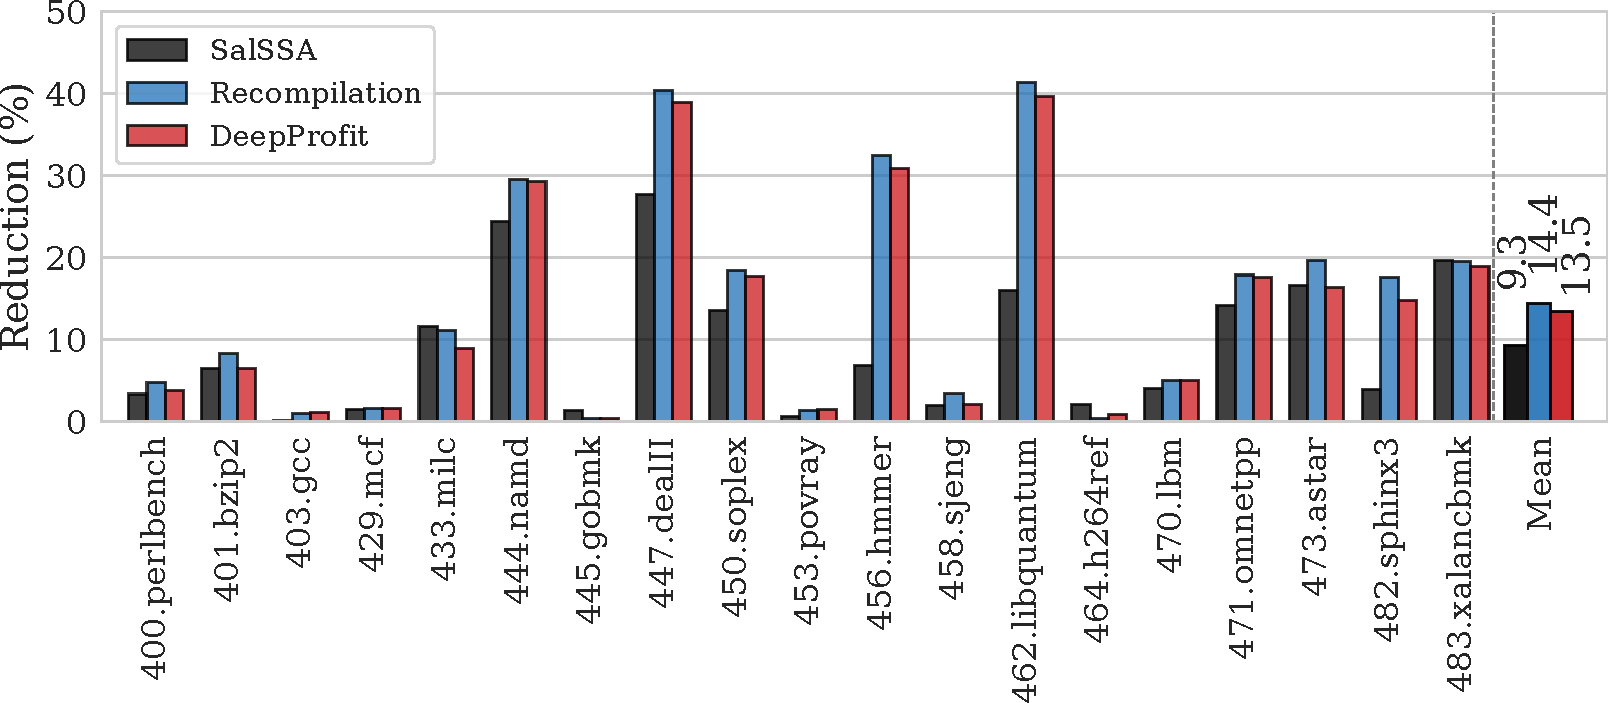
\includegraphics[width=0.85\textwidth]{src/deeplearning/figs/code-size-reduction-threshold-tuning.pdf}
  \caption{.}
  \label{fig:code-size-reduction}
\end{figure*}


%\begin{figure*}[h]
%  \centering
%  \includegraphics[width=0.7\textwidth]{src/deeplearning/figs/skipped-attempts.pdf}
%  \vspace{-2.5em}
%  \caption{.}
%  \label{fig:skipped-attempts}
%\end{figure*}

\begin{figure}[h]
  \centering
  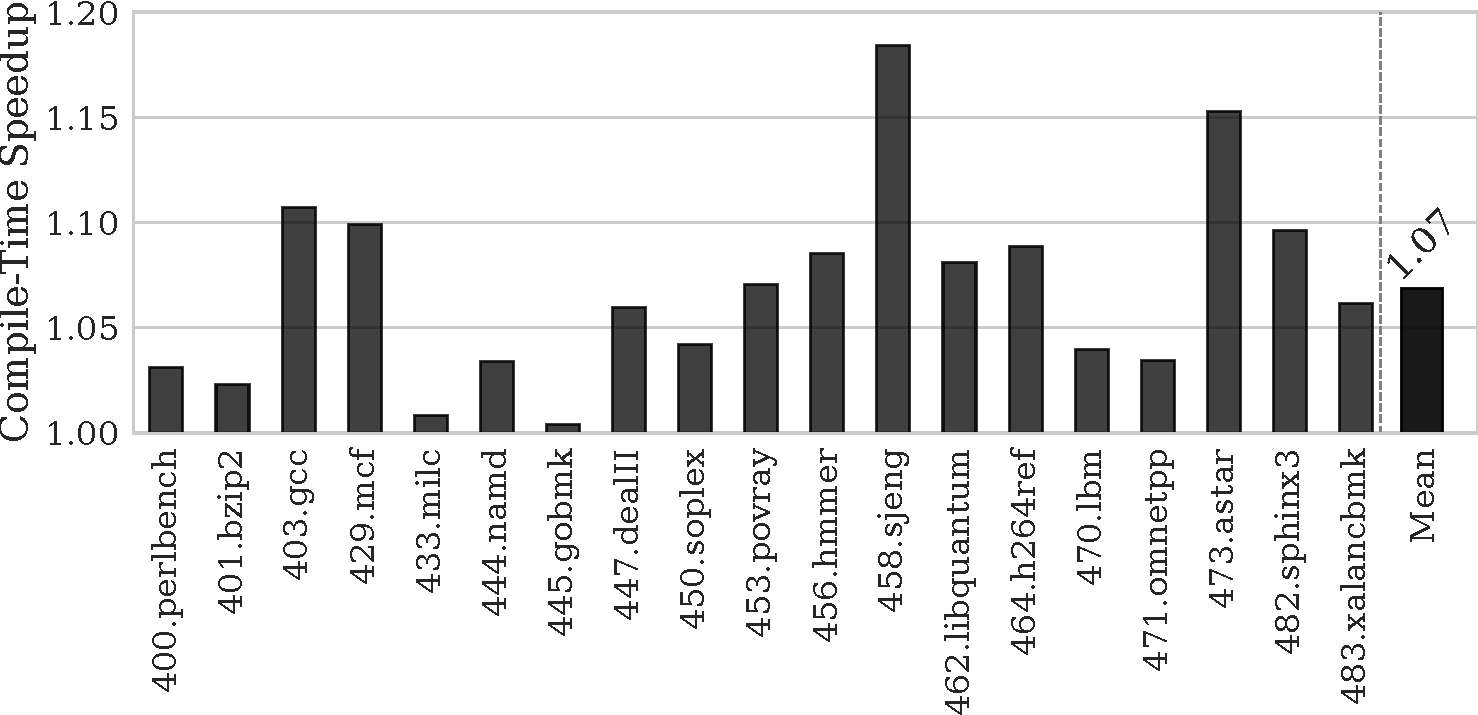
\includegraphics[width=0.95\textwidth]{src/deeplearning/figs/compilation-time-speedup.pdf}
  \caption{Compilation-time speedup over the version using partial recompilation.}
  \label{fig:compilation-time-speedup}
\end{figure}

